\section{Auswertung}
\label{sec:Auswertung}

\begin{table}
  \centering
  \caption{Messung der Biegung des runden Stabs bei einseitiger Einspannung}
  \label{tab:runds}
  \sisetup{table-format=2.1}
  \begin{tabular}{S[table-format=4.0] S[table-format=4.0]}
    \toprule
    {$x \mathbin{/} \si{\milli\meter}$} & {$D(x) \mathbin{/} \si{\milli\meter}$}\\
    \midrule
    100 & 0,28\\
    125 & 0,35\\
    150 & 0,36\\
    175 & 0,45\\
    200 & 0,51\\
    225 & 0,62\\
    250 & 0,78\\
    275 & 0,93\\
    300 & 1,16\\
    325 & 1,34\\
    350 & 1,58\\
    370 & 1,78\\
    400 & 2,07\\
    425 & 2,30\\
    450 & 2,58\\
    475 & 2,79\\
    500 & 3,10\\
    525 & 3,48\\
    \bottomrule
  \end{tabular}
\end{table}

\begin{table}
  \centering
  \caption{Messung der Biegung des runden Stabs bei beidseitiger Auflage}
  \label{tab:rundb}
  \sisetup{table-format=2.1}
  \begin{tabular}{S[table-format=4.0] S[table-format=4.0]}
    \toprule
    {$x \mathbin{/} \si{\milli\meter}$} & {$D(x) \mathbin{/} \si{\milli\meter}$}\\
    \midrule
    100 & 0,22\\
    125 & 0,25\\
    150 & 0,31\\
    175 & 0,30\\
    200 & 0,42\\
    225 & 0,38\\
    250 & 0,40\\
    275 \\
    300 & 0,40\\
    325 & 0,37\\
    350 & 0,41\\
    375 & 0,30\\
    400 & 0,31\\
    425 & 0,25\\
    450 & 0,21\\
    475 & 0,17\\
    500 & 0,12\\
    525 & 3,48\\
    \bottomrule
  \end{tabular}
\end{table}

\begin{table}
  \centering
  \caption{Messung der Biegung des eckigen Stabs bei einseitiger Einspannung}
  \label{tab:ecks}
  \sisetup{table-format=2.1}
  \begin{tabular}{S[table-format=4.0] S[table-format=4.0]}
    \toprule
    {$x \mathbin{/} \si{\milli\meter}$} & {$D(x) \mathbin{/} \si{\milli\meter}$}\\
    \midrule
    100 & 0,32\\
    125 & 0,46\\
    150 & 0,62\\
    175 & 0,73\\
    200 & 0,87\\
    225 & 1,03\\
    250 & 1,15\\
    275 & 1,32\\
    300 & 1,64\\
    325 & 1,86\\
    350 & 2,01\\
    375 & 2,32\\
    400 & 2,68\\
    425 & 2,90\\
    450 & 3,05\\
    475 & 3,44\\
    500 & 3,75\\
    \bottomrule
  \end{tabular}
\end{table}


\begin{table}
  \centering
  \caption{Messung der Biegung des eckigen Stabs bei beidseitiger Auflage}
  \label{tab:eckb}
  \sisetup{table-format=2.1}
  \begin{tabular}{S[table-format=4.0] S[table-format=4.0]}
    \toprule
    {$x \mathbin{/} \si{\milli\meter}$} & {$D(x) \mathbin{/} \si{\milli\meter}$}\\
    \midrule
    50 & 0,01\\
    75 & 0,03\\
    100 & 0,06\\
    125 & 0,07\\
    150 & 0,08\\
    175 & 0,11\\
    200 & 0,14\\
    225 & 0,15\\
    250 & 0,16\\
    275 \\
    300 & 0,18\\
    325 & 0,17\\
    350 & 0,16\\
    375 & 0,15\\
    400 & 0,12\\
    425 & 0,12\\
    450 & 0,10\\
    475 & 0,08\\
    500 & 0,04\\
    \bottomrule
  \end{tabular}
\end{table}

\begin{figure}
  \centering
  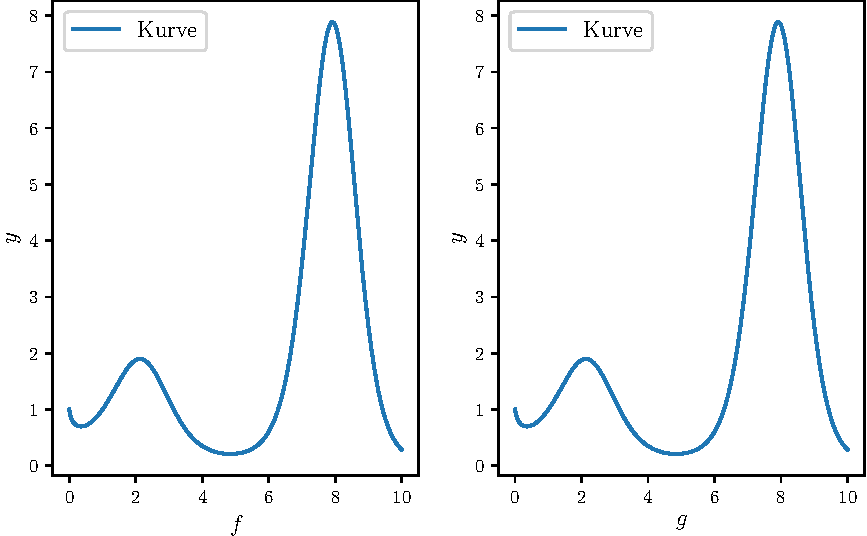
\includegraphics{plot.pdf}
  \caption{Plot.}
  \label{fig:plot}
\end{figure}


Siehe \autoref{fig:plot}!
